\documentclass[10pt]{article}

% Language setting
% Replace `english' with e.g. `spanish' to change the document language
\usepackage[english]{babel}

% Set page size and margins
% Replace `letterpaper' with`a4paper' for UK/EU standard size
\usepackage[a4paper,top=2cm,bottom=2cm,left=3cm,right=3cm,marginparwidth=1.75cm]{geometry}

% Useful packages
\usepackage{amsmath}
\usepackage{tikz}
\usepackage{graphicx}
\usepackage{mwe}
\usepackage{fullpage}
\usepackage{hyperref}
\hypersetup{linkcolor=blue, urlcolor=blue, colorlinks}
\usepackage{caption}
\usepackage{subcaption}
\usepackage{float}
\usepackage{enumerate}

\title{Project: Sparse Matrix Formats \\ \large \textit{Accelerator-based Programming}}
\author{Oskar Tegby}
\date{November 2022}

\setlength{\parindent}{0pt}

\begin{document}
\maketitle

\begin{tikzpicture}[remember picture, overlay]
  \node [anchor=north west, inner sep=25pt]  at (current page.north west)
     {
\includegraphics[height=3.3cm]{uppsala-universitet-logo.png}};
\end{tikzpicture}

\section{Introduction}
This project studies the computational bandwidths of an iterative solver for a finite element problem using a data structure for sparse matrices called compressed row storage (CRS). To be specific, we study the computational throughput of a conjugate gradient method with a sparse matrix that comes from the finite element discretization of the Laplacian on a three-dimensional domain $(0,1)^3$ meshed with bricks. Notably, this problem is studied both on the processor using C++ and on the graphics card using CUDA. \\

All tests were run on the \href{https://www.uppmax.uu.se/resources/systems/the-snowy-cluster/}{Snowy} node of the UPPMAX cluster using a NVIDIA Tesla T4 graphics card, an Intel Xeon E5-2660 processor, and were repeated 50 times to reduce the noise in the measurements.

\section{Tasks}
This section addresses the grading criteria to pass the assignment one-by-one in order to clearly show that the required functionality and knowledge has been obtained.
\subsection{Criteria 1}
\subsubsection{Instruction}
\textit{Provide a correct program for the basic tasks involving the CRS matrix both on the CPU and the GPU.}
\subsubsection{Solution}
Please find the attached code. The correctness of these implementations is assured by observing that the error of the $\ell^2$ norm decreases by a factor four when doubling the problem size, $N$, when executing the code. This is done by running the executable in the following way
\begin{center}
    \texttt{/app.v -repeat 100 -number Number},
\end{center}
where \texttt{Number} refers to the datatype used, which is either \texttt{float} or \texttt{double}, and \texttt{v} refers to either the \texttt{host} or \texttt{cuda} code. By running the code with either option we indeed fine that that is the case.
\subsection{Criteria 2}
\subsubsection{Instruction}
\textit{Provide computational measurements of acceptable performance on both platforms and display them in an understandable manner.}
\subsubsection{Solution}
Please refer to Figure \ref{fig:cpu} and Figure \ref{fig:gpu} for the CPU and GPU results, respectively.
\begin{figure}[!ht]
        \centering
    \begin{subfigure}[b]{0.49\textwidth}
        \centering
        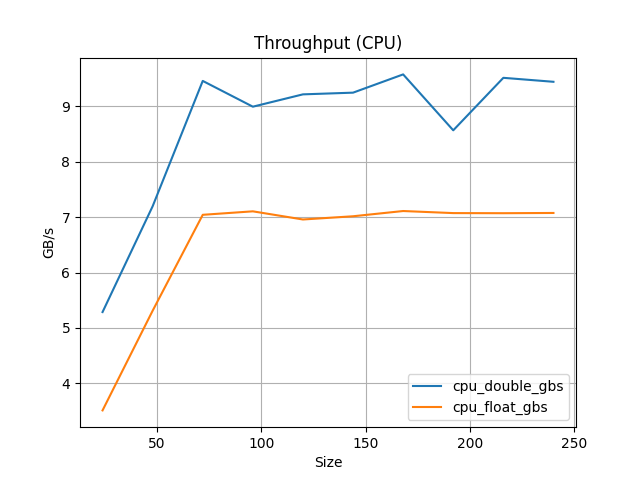
\includegraphics[width=\linewidth]{figs/cpu_gbs.png}
        \caption{The CPU throughput in GB/s.}
        \label{fig:cpu_gbs}
    \end{subfigure}\hfill
    \begin{subfigure}[b]{0.49\textwidth}
        \centering
        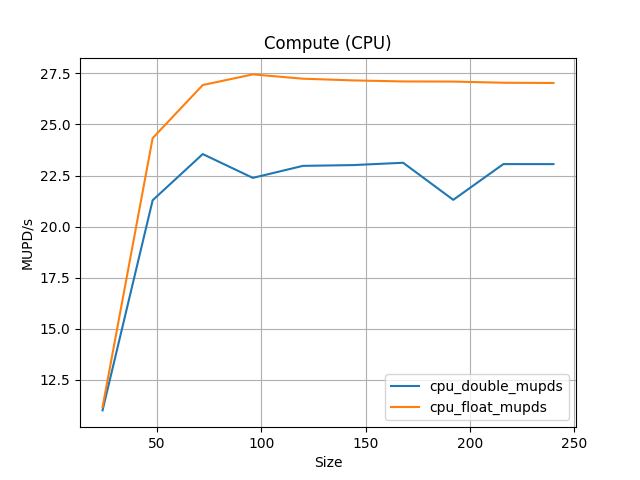
\includegraphics[width=\linewidth]{figs/cpu_mupds.png}
        \caption{The CPU compute in MUPD/s.}
        \label{fig:cpu_mupds}
    \end{subfigure}\hfill
    \caption{The throughput and compute achieved on the CPU.}
    \label{fig:cpu}
\end{figure}
\begin{figure}[!ht]
        \centering
    \begin{subfigure}[b]{0.49\textwidth}
        \centering
        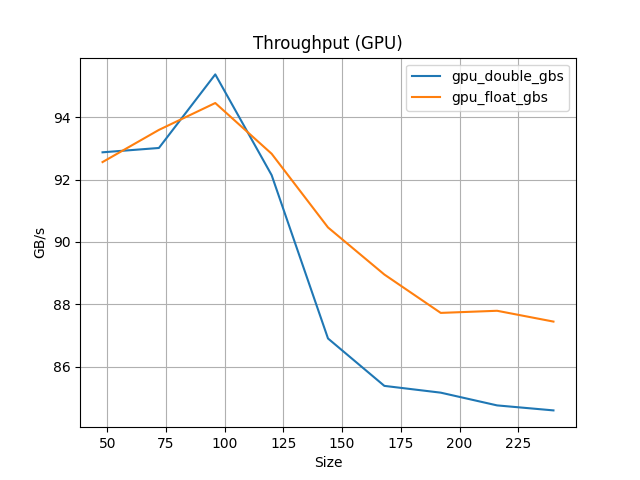
\includegraphics[width=\linewidth]{figs/gpu_gbs.png}
        \caption{The GPU throughput in GB/s.}
        \label{fig:gpu_gbs}
    \end{subfigure}\hfill
    \begin{subfigure}[b]{0.49\textwidth}
        \centering
        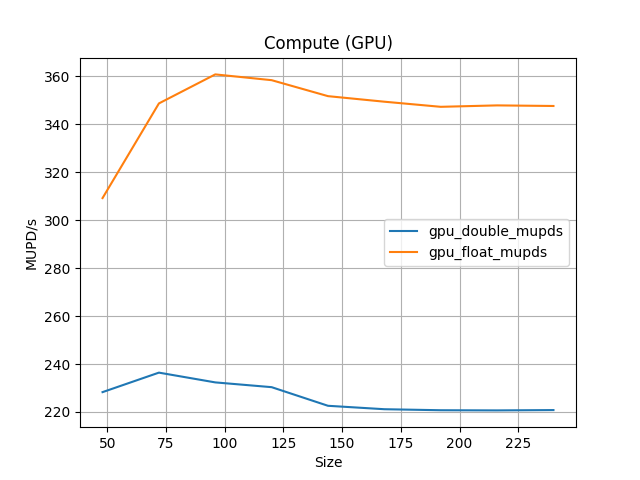
\includegraphics[width=\linewidth]{figs/gpu_mupds.png}
        \caption{The GPU compute in MUPD/s.}
        \label{fig:gpu_mupds}
    \end{subfigure}\hfill
    \caption{The throughput and compute achieved on the GPU.}
    \label{fig:gpu}
\end{figure}
\subsection{Criteria 3}
\subsubsection{Instruction}
\textit{Provide explanations for the expected performance of the sparse matrix-vector product and conjugate gradient solver with basic CRS matrix storage as well as the improved ELLPACK/SELL-C-Sigma approach by Kreutzer et al.}
\subsubsection{Solution}
The performance with basic CRS storage is poor since the potential performance gained by vectorization and parallelization of the matrix-vector multiplication is ruined by the irregular data storage. That is solved by the ELLPACK storage, which fills all of the rows with zeros so that the rows are the same length. \\

However, that introduces the issue of potentially storing a lot of unnecessary zeros, which CELL-C-$\sigma$ solves by locally sorting $\sigma$ rows of the data. That is, the data is sorted in groups of $\sigma$ elements. The C in SELL-C-$\sigma$ indicates how large the groups which are given extra zeros are. This decreases the number of zeros substantially, which improves performance without losing the ability to easily vectorize and parallelize the implementation, which means that it still is suitable to run on the GPU. \\

The expected performance increase from CRS to ELLPACK/SELL-C-$\sigma$ should be about a factor two to three given the greatly improved data-access patterns. The reason is that it will be possible to vectorize the computations, which, from experience, only reach about half of the theoretical performance increase due to the overhead of packing the vectors. Furthermore, it is, in general, easier to split the work between threads when the amount of work each thread needs to perform is easily predictable. \\

The cache hit-rate will also be higher since we will be able to prefetch data by having a more regular data-access pattern, which is required in order for the prefetcher to be able to do a good job at prefetching in order to hide the memory latency. This behavior should not differ much between ELLPACK and SELL-C-$\sigma$ since both have evened out the arrays by adding zeros to varying extents. The only noticable difference is that we will be loading a lot of padding zeros for ELLPACK, which will cause unnecessary loads to be issued, which causes unnecessary delays. Notably, the latter will become more noticable the larger the arrays get and the more uneven the rows are. \\

Regarding the performance for the sparse matrix-vector product and conjugate gradient solver in particular, there is no reason to believe that the nature of the matrix operations would matter since the only thing that matters is the speed of which we can load and store data in the matrices (as well as the largest-feasible problem size).  
\subsection{Criteria 4}
\subsubsection{Instruction}
\textit{Discuss the topics of data both in the report and during oral discussion of the project.}
\subsubsection{Solution}
The answer to Criteria 3 has already touched on the topic of data storage to some extent. Although not mentioned explicitly as criteria here, it is worthwhile to consider the different nature of desirably memory memory distribution on CPUs and on GPUs. \\

Namely, on CPUs we want each thread to access memory contiguously, and to work on different parts of the memory in order to use the CPU efficiently. The reason is that each thread, ideally, should be running on different cores so that they have private access to the $L1$ cache, so that they can use as much of it as possible in order to perform computations (assuming that we need to use all of the L1 cache). Perhaps more importantly, we want the threads to access one cacheline and perform operations on all of it, ideally using vector instructions doing so. Thus, we want to run every thread on different parts of the computation. \\

On GPUs, however, the contrary is true since one thread will load data to the shared memory, allowing the rest of the threads to perform computations on it as well. If we assign one thread per memory access, then they will all load data to their shared memory with only one thread computing on it at a time. The idea is that we want to access memory at the loaded at the same time. \\

In this context, we would most likely want to run parallelize ELLPACK by splitting up the number of rows among the threads both for the CPU and for the GPU. Naturally, we would also like to coalesce the memory access on the GPU, and keep them contiguous on the CPU. \\

None of this should prove any challenge here, except the potential problem of keeping one warp busy running on short lines, since many of the threads would stall when the amount of work is less than the number of threads in the warp. Along the same lines, it would be hard to keep enough warps busy on one streaming multiprocessor if the work is not allocated in some clever way. That is to say that it would be easy to run into the issue of getting stalled threads. \\

On the CPU, this should not become an issue since we would simply spread the rows on each processor. Arguably, the same could be done on the GPU, but then we would need to split the work between the streaming multiprocessors such that we utilize the shared memory in order to speed up the local memory transfers. \\

Another question the is interesting to discuss here is about the roofline model. Namely, if we are compute or bandwidth bound in this setting. Given that we only reach about 80-100 GB/s it should be clear that we are bandwidth-bound since we are not maxing out the bandwidth to the main memory on the graphics card. If we were to do so, then we would see that increasing the problem size would simply keep us that the maximum throughput that we could achieve. \\

Naturally, we would not need to reach the bandwidth of the graphics memory before that would happen since we always have to expect some overhead or inefficiency of the hardware utilization for our implementation, such as not keeping all streaming multiprocessors running, accessing memory poorly, or running into divergent computing from a conditional statement. 
\subsection{Criteria 5 (Addition 1)}
\subsubsection{Instruction}
\textit{Determine if it is worth running the pipeline of the GPU. Measure the transfer time from the CPU to GPU and the total executon time.}
\subsubsection{Solution}
{\color{yellow}The code to record and render the results for this part is written, but as of submitting this document, it is not possible to claim a GPU node after having waited for two hours despite having been able to do so with ease just a few hours ago. Consequently, the necessary measurements cannot be obtained right now, but I will try again as soon as possible, and upload and answer to this question and notify you when that has been done. This should of course have been done earlier, for which I humbly apologize.}
% The overall execution times and the transfer time from the CPU to the GPU is found for single precision in Figure A and for double precision in Figure B. There, we observe that the transfer time from the CPU to the GPU constitutes a significant time of the entire execution time, which we assume is greater than the time saved by running the kernel on the GPU instead of on the CPU. However, in order to verify this properly, we would need to run the multithreaded version on the CPU, but that is currently impossible due to issues getting OpenMP to run for this code.
%\begin{figure}[!ht]
%        \centering
%    \begin{subfigure}[b]{0.49\textwidth}
%        \centering
%        \includegraphics[width=\linewidth]{figs/float_execution_times.png}
%        \caption{The execution times with single precision.}
%        \label{fig:single_times}
%    \end{subfigure}\hfill
%    \begin{subfigure}[b]{0.49\textwidth}
%        \centering
%        \includegraphics[width=\linewidth]{figs/double_execution_times.png}
%        \caption{The execution times with double precision.}
%        \label{fig:double_times}
%    \end{subfigure}\hfill
%    \caption{The total execution time and the transfer time from the CPU to the GPU.}
%    \label{fig:times}
%\end{figure}
\subsection{Criteria 6 (Addition 2)}
\textit{Relate the CUDA code to a framework-based solution with Kokkos or similar, and discuss possible limitations in terms of the data layout possible with multi-dimensional arrays.}
\subsubsection{Solution}
It would be possible to create a view in Kokkos where we store the data in a two-dimensional array. This works well for ELLPACK since it has two dimensions: The number of non-zero rows and the length of the longest padded row of non-zero elements. However, this will not work as well for CELL-C-$\sigma$ since we will not be able to create blocks of different sizes without creating one view for every combination of block dimensions. It could of course be done in theory, but it would require a lot of micro-managing the computations, which is contrary to the idea of Kokkos. It would most likely be simpler to just write the code in CUDA, where we could focus on making a custom data structure or routine which suits our needs much better.
\end{document}
